let us consider a function $z=f(x, y)$ which has a local maximum at
$(a,b)$.  We know that this implies that $(a,b)$ is a critical point
for $f$, so that
\[
\pdd fx(a,b) = \pdd fy(a,b) = 0.
\]
Now look at the function of one variable
\[
g(x) \stackrel{\rm def}= f(x, b)
\]
which you get by freezing $y$ at the value $b$.  Since $f(x,y)$ has a
local maximum at $(a, b)$ the function $g(x)$ has a local maximum at
$x=a$.  From one-variable calculus we know that 
\[
g'(a) =0 \text{ and } g''(a)\leq 0.
\]
The derivatives of $g$ are
\[
g'(x) = f_x(x, b), \qquad g''(x) = f_{xx}(x, b).
\]
So we find that $g'(a) = 0$ implies $f_x(a, b) = 0$, which we already
knew, and $g''(a)=0$ implies
\begin{equation}
  f_{xx}(a, b) \leq 0.
  \label{eq:03fxx-nonpositive}
\end{equation}
Conclusion: \emph{if $f(x, y)$ has a local maximum at $(a, b)$, then
$f_{xx}(a,b) \le 0$.}

By freezing $x$ instead of $y$ and looking at the function 
\[
h(y) = f(a, y)
\]
the same reasoning tells you that $h'(b) = f_y(a, b)=0$, which we already
knew, and $h''(b) = f_{yy}(a, b)\leq 0$.

Combined with our previous conclusion we have discovered the
following: \emph{if $f$ has a local maximum at $(a, b)$, then}
\begin{equation}\label{eq:03not-the-2nd-deriv-test}
  f_{xx}(a, b) \leq 0 \text{ and } f_{yy}(a, b) \leq 0
\end{equation}
\emph{must hold}.  This suggests that the two-variable version of the
second derivative test could be something like this: to see if a
critical point $(a,b)$ is a local maximum, you compute $f_{xx}(a, b)$
and $f_{yy}(a, b)$ and then check if they are negative.
Unfortunately, \emph{this is the wrong test!} While
\eqref{eq:03not-the-2nd-deriv-test} must hold at any local maximum of
$f$, the converse turns out not to be true: if
\eqref{eq:03not-the-2nd-deriv-test} holds at some critical point $(a,
b)$ of a function $f$, then $(a, b)$ need not be a local maximum of
$f$.

The following example shows what can go wrong.

\subsection{An example of a function that doesn't have a local 
  maximum, even though it satisfies \eqref{eq:03not-the-2nd-deriv-test}}
\label{sec:03not-a-local-max}
The function
\[
f(x, y) = 4xy-x^2-y^2
\]
has the following partial derivatives at the origin:
\[
f_x(0,0) = f_y(0,0) = 0,
\qquad
f_{xx}(0,0) = f_{yy}(0,0) = -2.
\]
The origin is a critical point:  could it be a local maximum?  When we 
check to see if \eqref{eq:03not-the-2nd-deriv-test} applies we see
that it does.  Indeed, to elaborate on this, note that freezing $y=0$
gives you the function
\[
g(x) = f(x, 0) = -x^2
\]
which has a global maximum at $x=0$, and freezing $x=0$ leads you to
the function
\[
h(y) = g(0,y) = -y^2
\]
which also has a global maximum at $y=0$.  If we believed that
\eqref{eq:03not-the-2nd-deriv-test} really were a good second
derivative test, then we would now think that the function $f$ has a local
maximum at the origin, meaning that for $(x, y)$ close to $(0,0)$ we would
expect $f(x,y) < 0$.
But if you compute $f(x, y)$ along the line $y=x$ you find 
\[
f(x, y) = f(x,x) = 4xx-x^2-x^2 = +2x^2.
\]
So along the line $y=x$ the function is positive, and $f$ therefore
cannot have a local maximum at the origin.

We have found an example of a function with a critical point that satisfies
\eqref{eq:03not-the-2nd-deriv-test}, but that doesn't have a local maximum
at the critical point.  See Figure~\ref{fig:03example-2nd-deriv-test}.

The example shows that even when the graph of a function is curved
downwards in both the $x$ and $y$ directions, it can still curve upwards in
other directions.  A good second derivative test should take this into
account, and because of this we need to know how to see that ``the graph
curves up/down in some direction.''

\begin{figure}[ht]
  \centering
  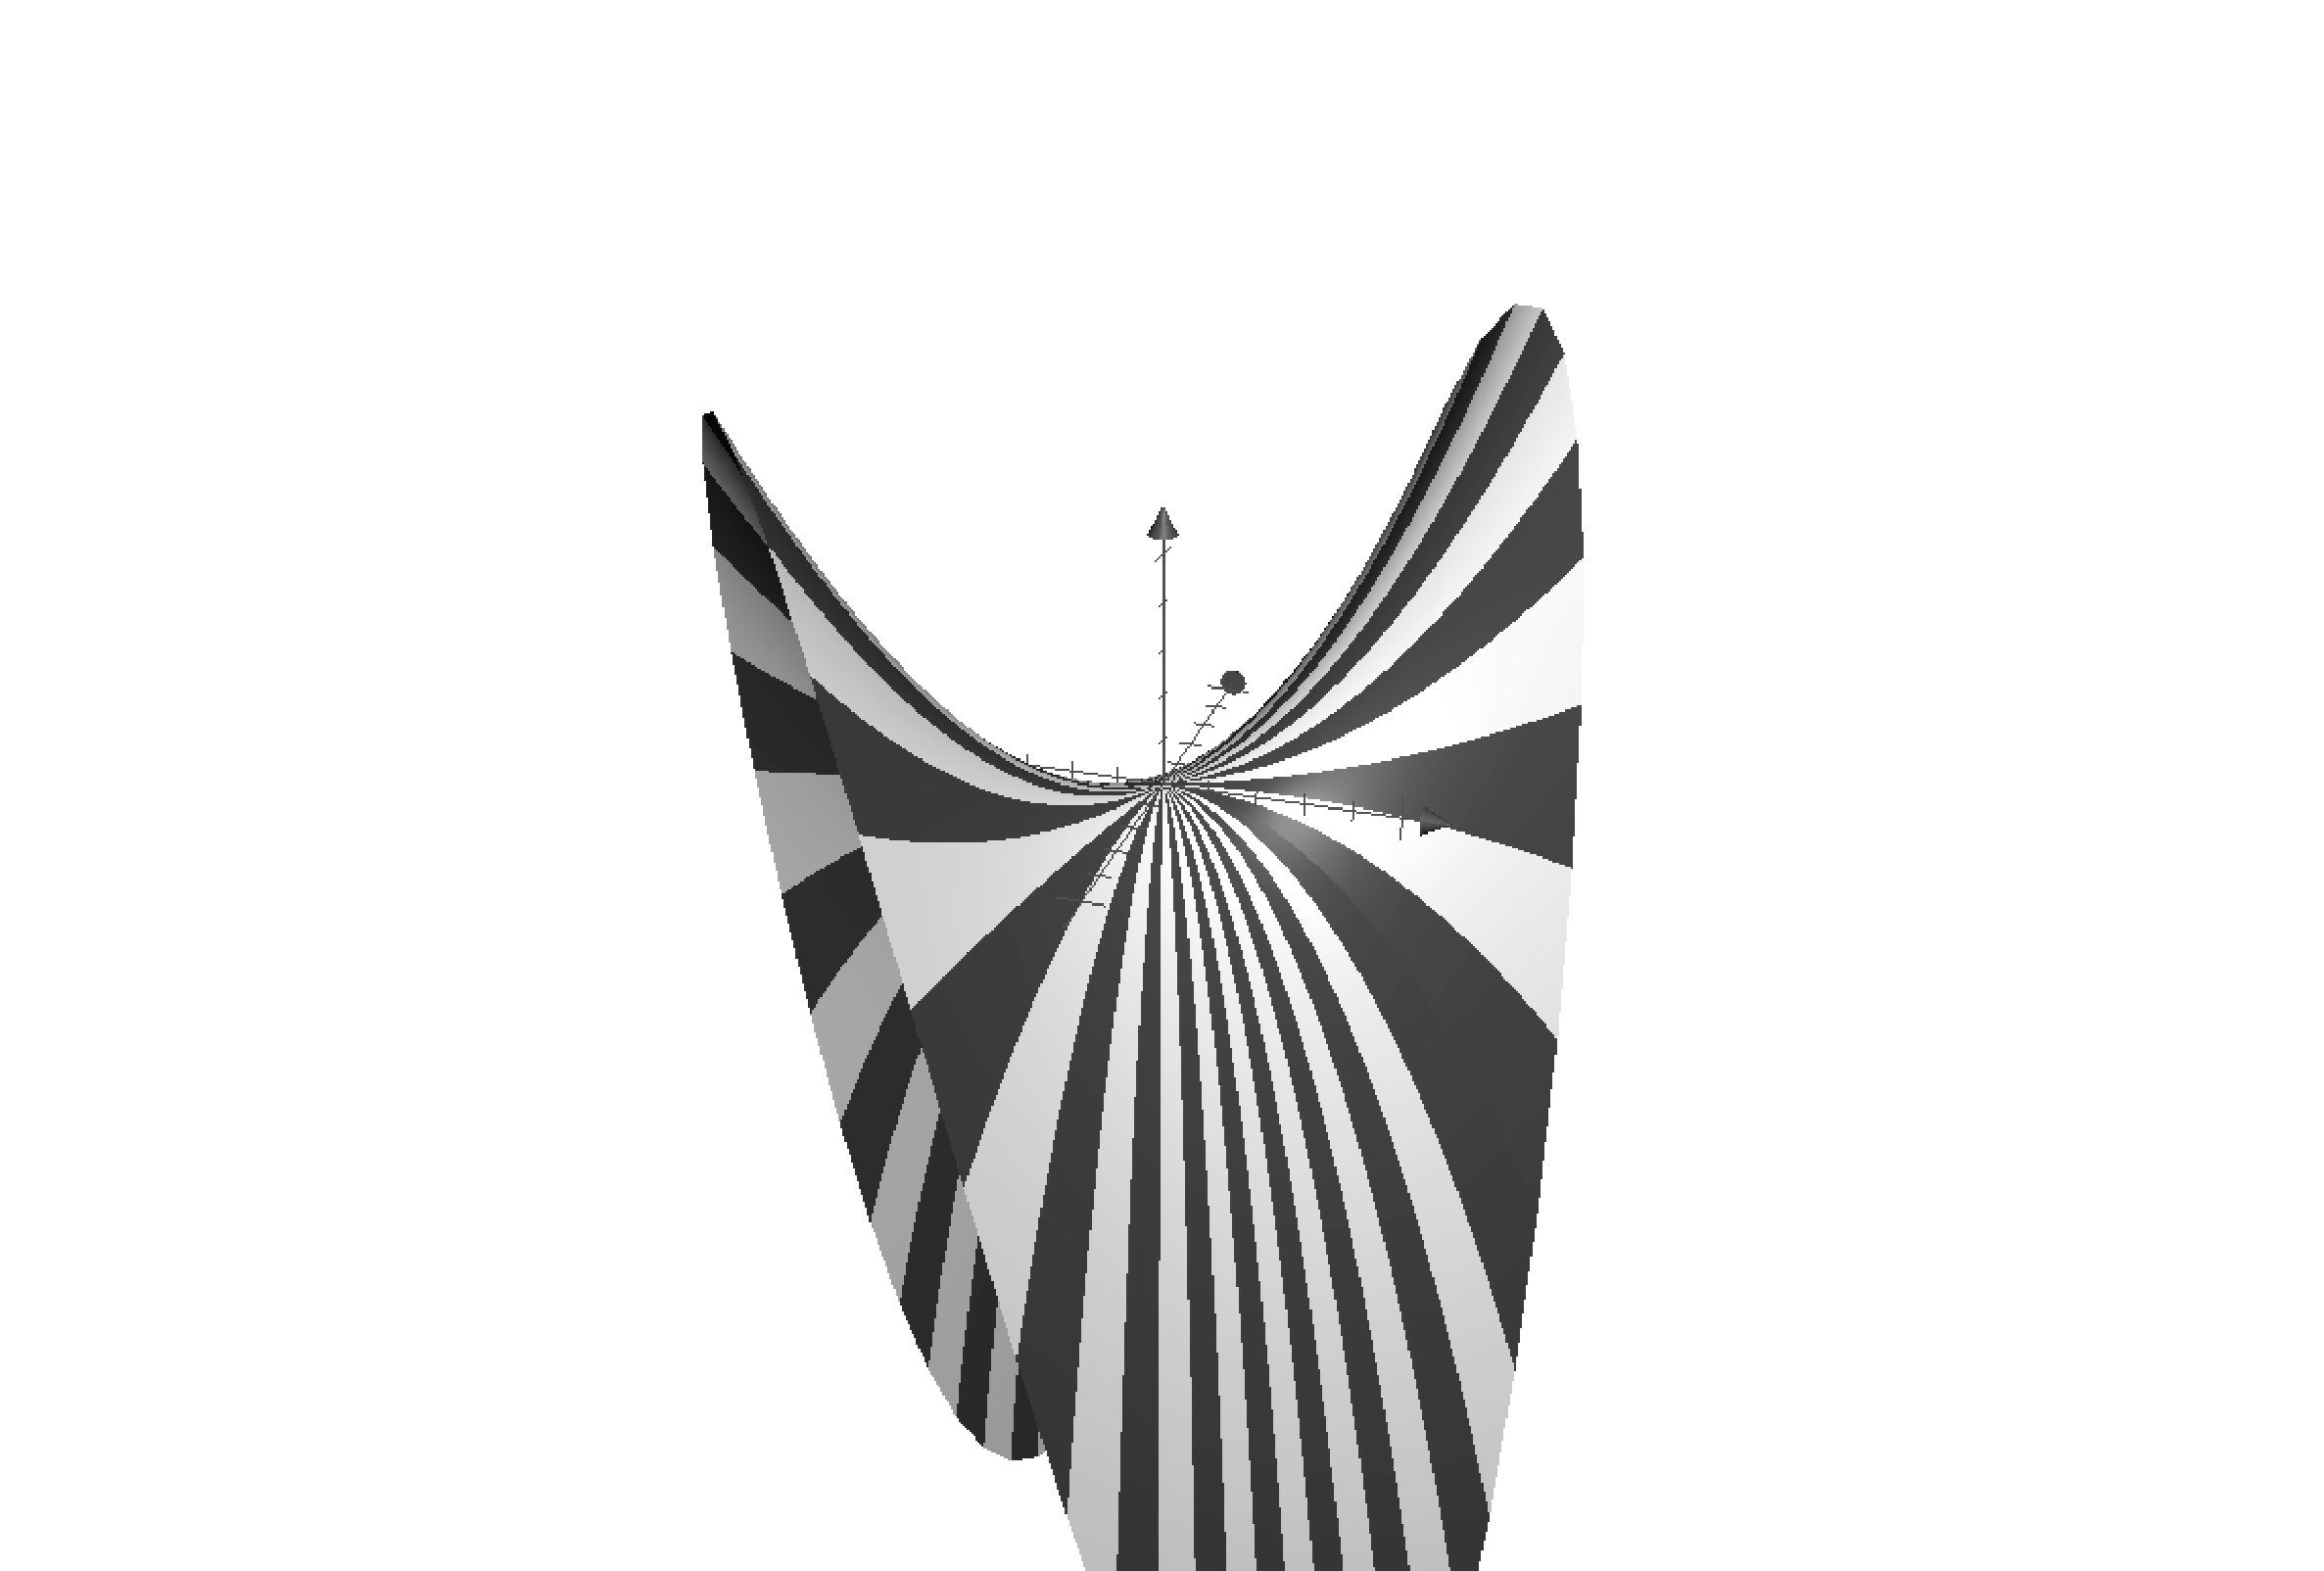
\includegraphics[width=0.3\textwidth]
      {figures/03example-2nd-deriv-test-a-bw.pdf}
  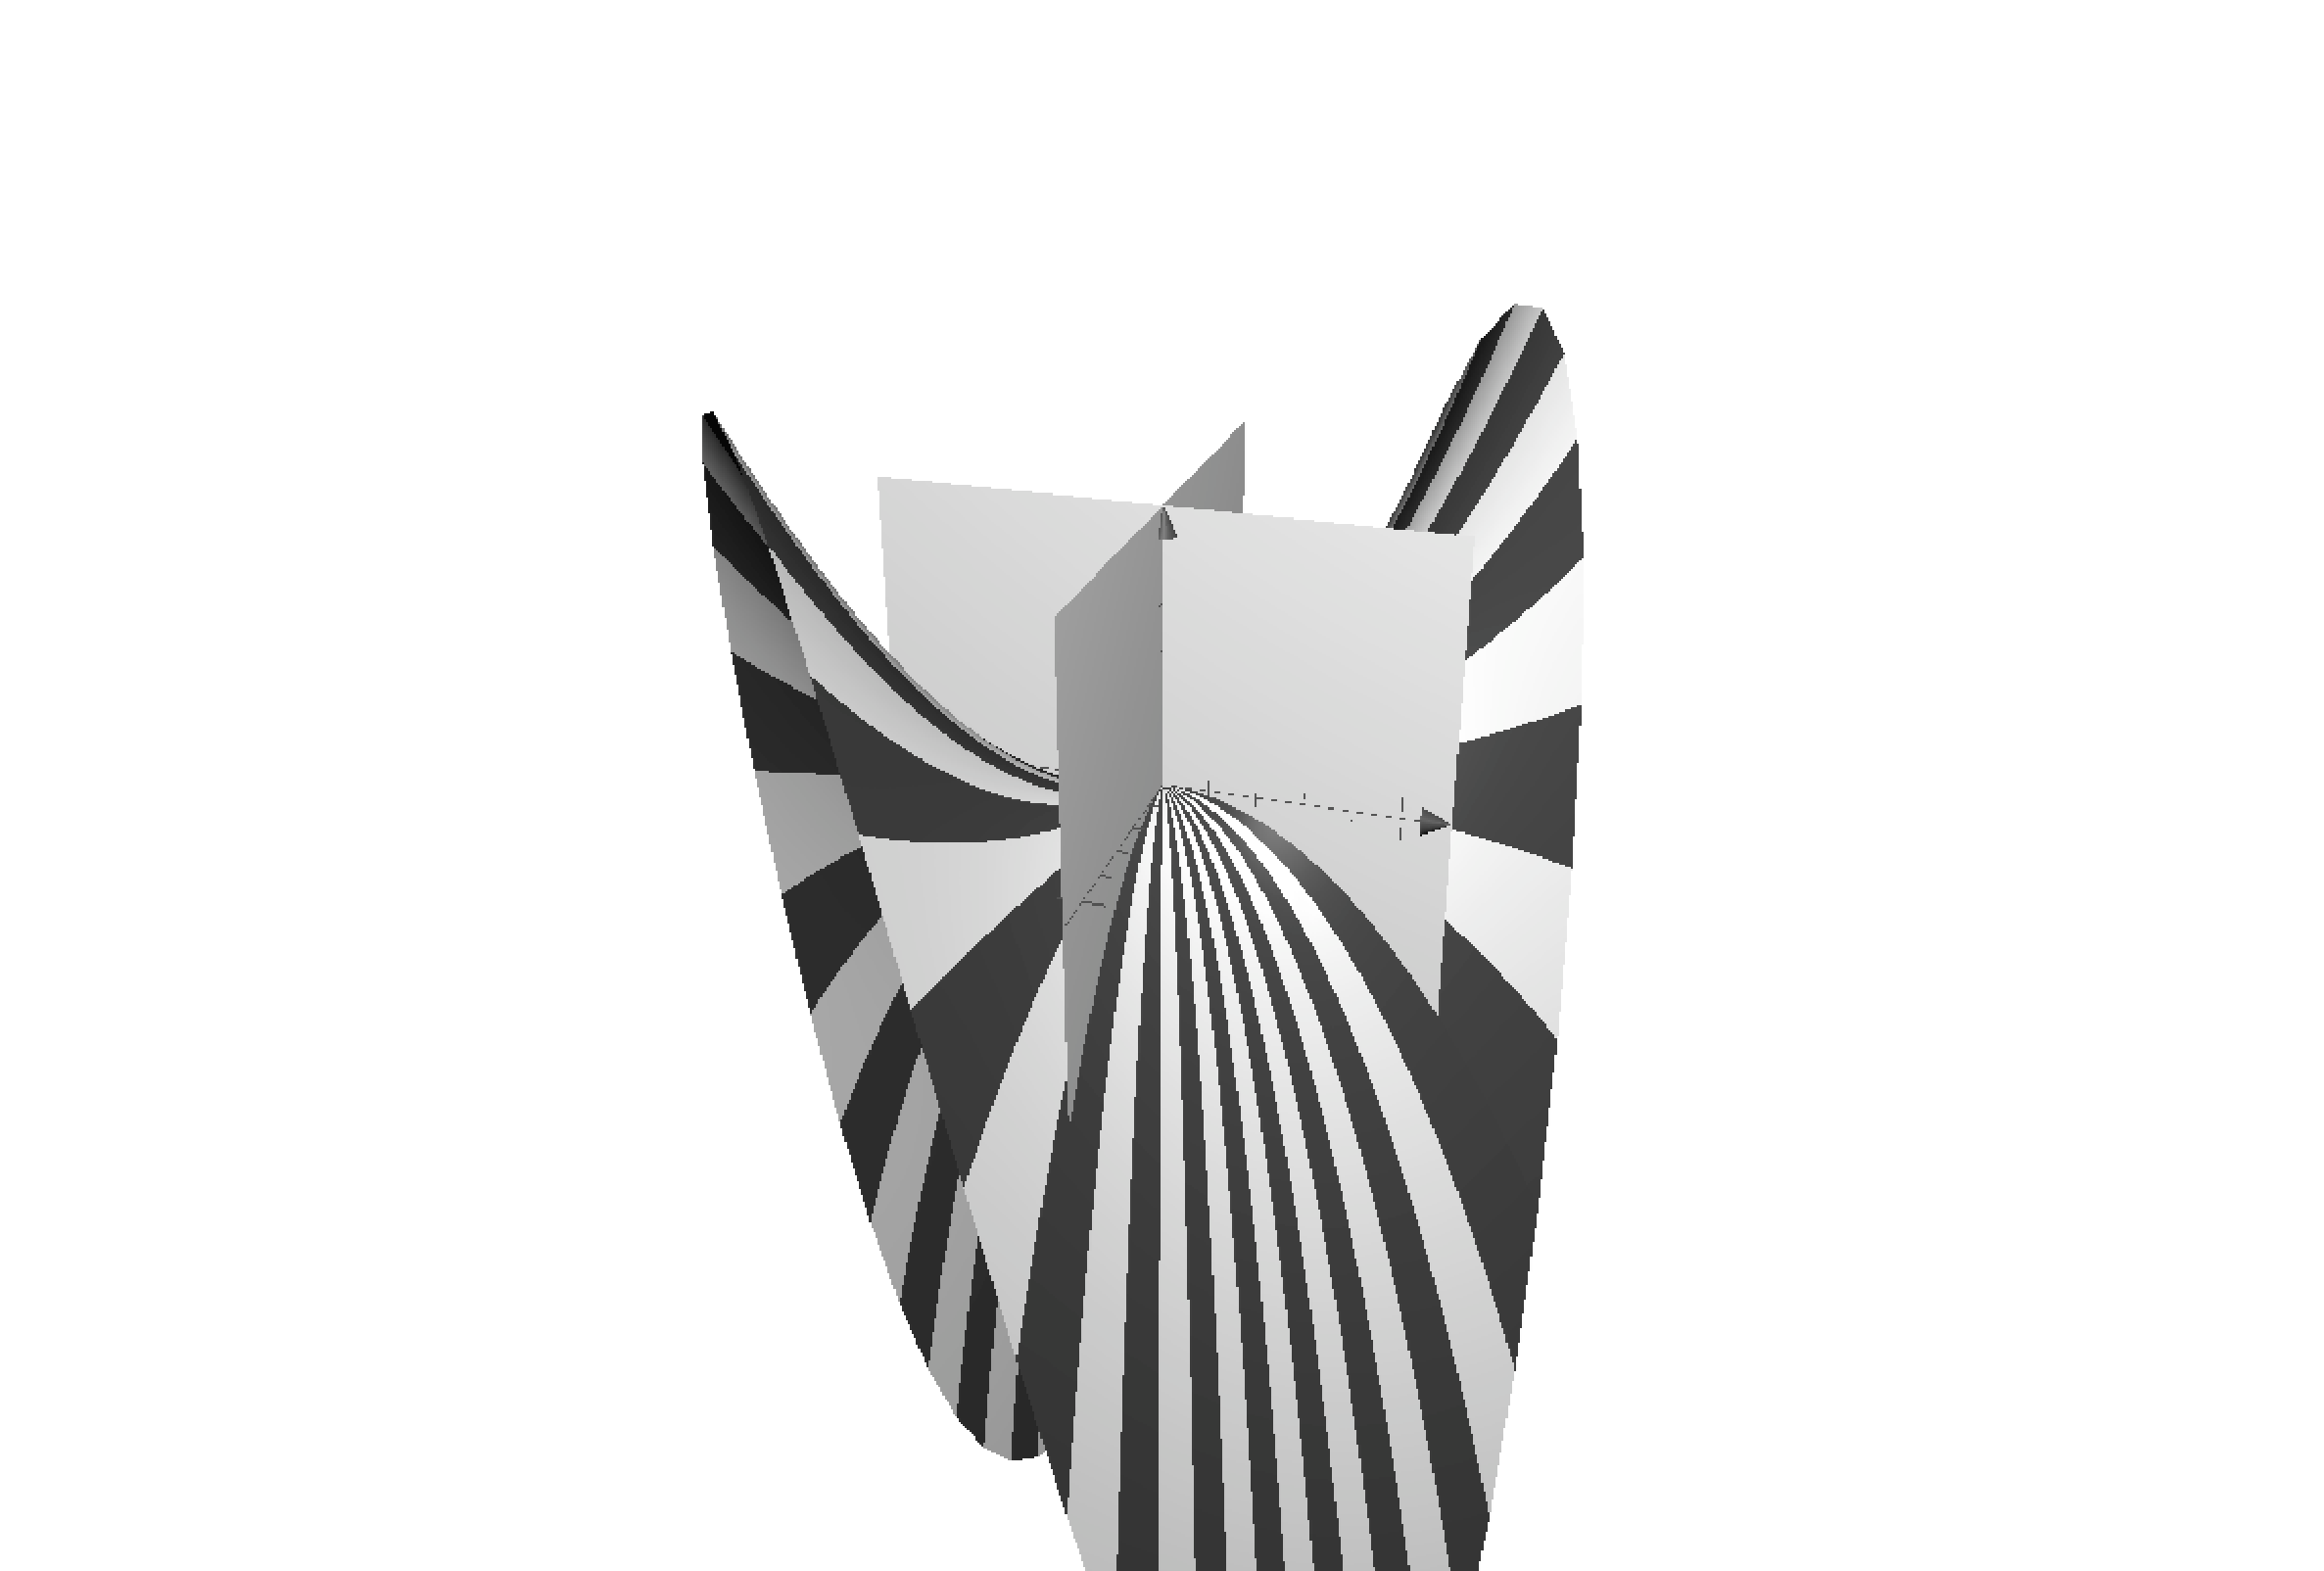
\includegraphics[width=0.3\textwidth]
      {figures/03example-2nd-deriv-test-b-bw.pdf}
  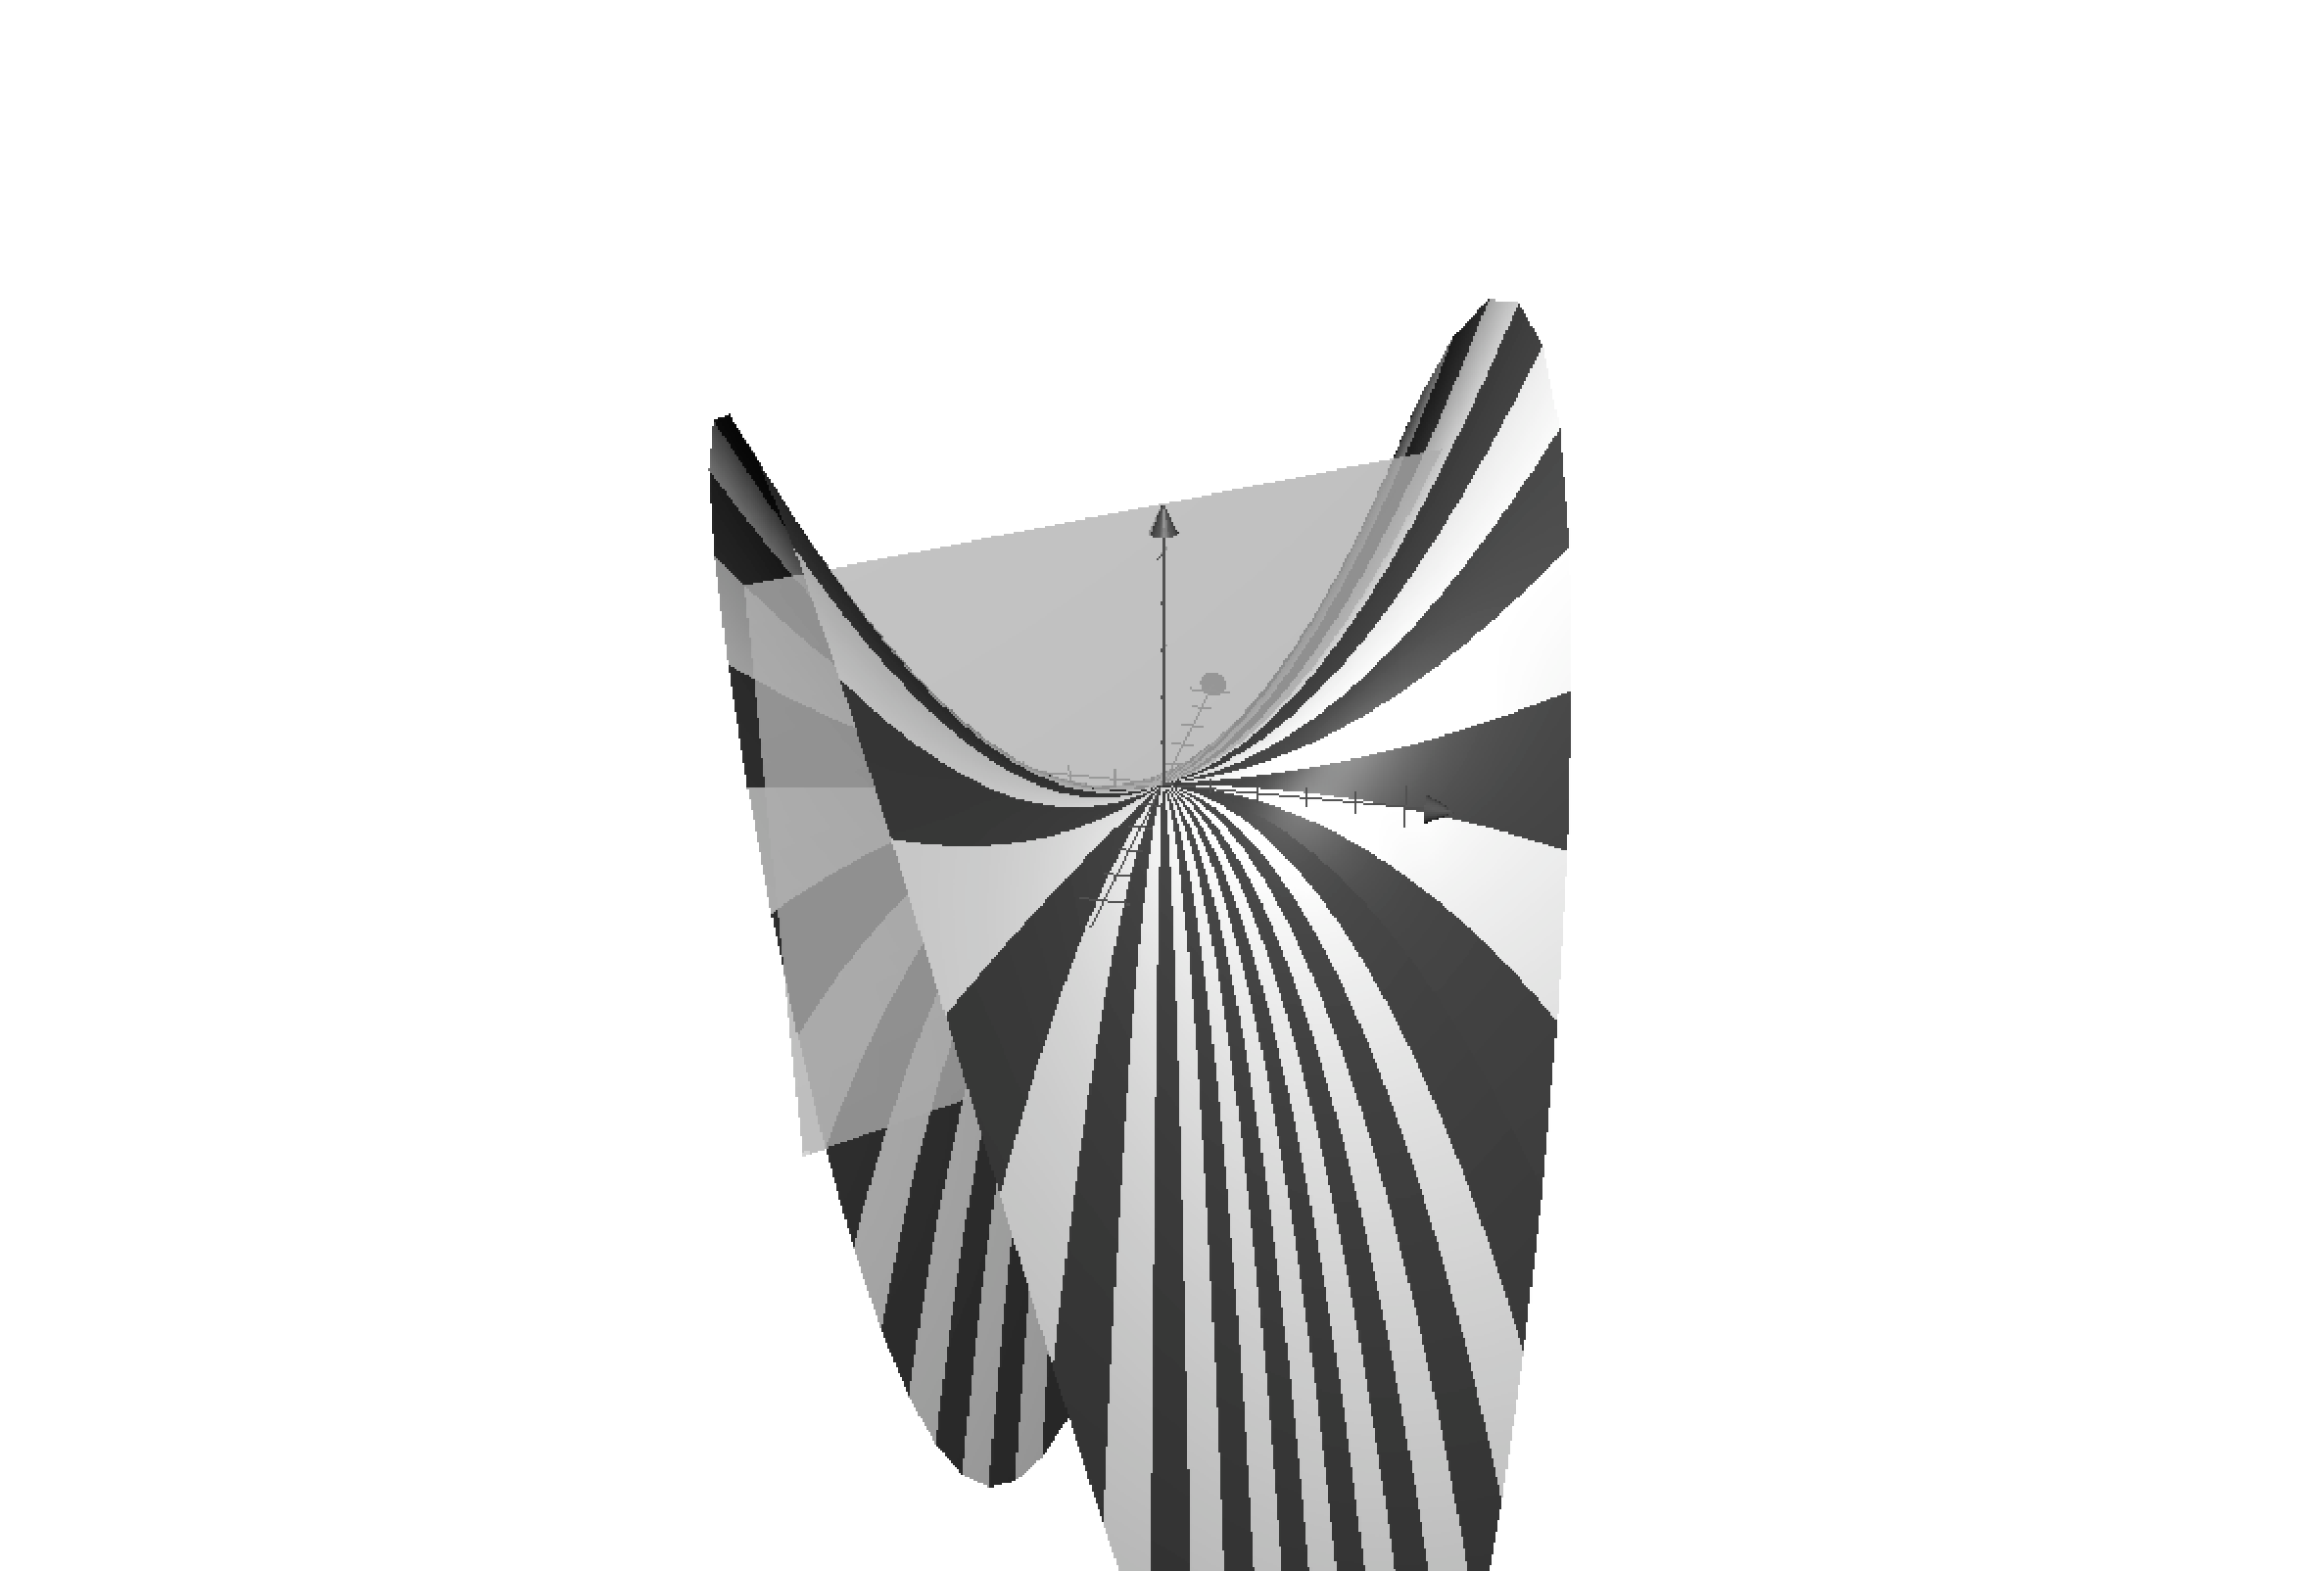
\includegraphics[width=0.3\textwidth]
      {figures/03example-2nd-deriv-test-c-bw.pdf}
  \caption{\textbf{On the left}, the graph of $z = f(x,y) =
  4xy-x^2-y^2$ from \S\ref{sec:03not-a-local-max}.  \textbf{Middle:}
  intersecting the graph with the planes $x=0$  and $y=0$  shows that
  both $f(x, 0)$ and $f(0, y)$ have local maxima at $x=0$, or $y=0$,
  respectively.  \textbf{Right:}  Intersection with the plane $y=x$
  shows that $f(t, t)$ has a local minimum at $t=0$.  Conclusion: this
  function satisfies the condition \eqref{eq:03not-the-2nd-deriv-test}
  at the origin, but it does not have a local maximum there.}

  \label{fig:03example-2nd-deriv-test}
\end{figure}

\subsection{The second derivative in any direction} 
\label{sec:second-deriv-in-any-direction}
Suppose we have a function $f$ with a critical point $(a,b)$ which
satisfies (\ref{eq:03not-the-2nd-deriv-test}).  Then the previous
example shows that even though the graph of $f$ is curved downwards in
the $x$ and in the $y$ directions, it may still be curved upwards in
other directions.

A good second derivative test will check that the graph of $f$ is
curved downwards in all directions.  To do this, we pick any two
numbers $m,n$ and consider the function
\begin{equation}
  \label{eq:function-on-line-through-cpt}
  g(t) \stackrel{\rm def}{=} f(a+mt, b+nt).
\end{equation}

\begin{figure}[b]
  \centering
  \includegraphics{figures/03second-variation.pdf}
  \caption{Computing the second derivative in the direction of a
  vector $\binom mn$}
  \label{fig:second-variation}
\end{figure}

If $f$ has a local maximum at $(a,b)$, then $g(t)$ must have a local
maximum at $t=0$.  First semester calculus implies $g'(0) = 0$ and
$g''(0)\leq 0$.  Using the chain rule you calculate the derivatives of
$g$, and you get
\begin{align*}
  g'(t) &= \frac{d f(a+mt, b+nt)}{dt} \qquad\text{(apply chain rule)}\\
  &= f_x(a+mt, b+nt) \frac{d (a+mt)}{dt}
  + f_y(a+mt, b+nt) \frac{d (b+nt)}{dt}\\
  &=  f_x(a+mt, b+nt) m + f_y(a+mt, b+nt) n.
\end{align*}
Differentiating again leads you to the second derivative of the
function $f$ along the line $\ell$
\begin{align*}
  g''(t) &= \frac{d^2 f(a+mt, b+nt)}{dt^2} \\
  & = f_{xx}(a+mt, b+nt) m^2 + 2
  f_{xy}(a+mt, b+nt) mn + f_{yy}(a+mt, b+nt) n^2.
\end{align*}
When you are computing this you get two terms with mixed second
derivatives, but because $f_{xy} = f_{yx}$, by Clairaut's theorem,
they combine to give us the $2f_{xy}$ term in the middle.

Finally we set $t=0$ to get
\begin{equation}
  g''(0) = \left.\frac{d^2 f(a+mt, b+nt)}{dt^2}\right|_{t=0} =
  f_{xx}(a,b) m^2 + 2f_{xy}(a,b) mn + f_{yy}(a,b)n^2.
  \label{eq:second-variation}
\end{equation}
We can think of this expression as the second derivative of the function
$f$ along the vector $\tvek m\\n\ttor$, or the second derivative of $f$
along the line through the point $(a,b)$ in the direction of the vector
$\tvek m\\n\ttor$.

We began this computation with the assumption that $f$ has a local maximum
at $(a,b)$, and concluded from this that $g''(0)\leq 0$, so our computation
shows that if $f$ has a local maximum at $(a,b)$, then 
\begin{equation}
  f_{xx}(a,b) m^2 + 2f_{xy}(a,b) mn + f_{yy}(a,b)n^2 \leq 0
\end{equation}
must hold for any choice of $m, n$.  It turns out that this is the correct
second derivative test:

\subsection{The second derivative test}
\label{sec:2nd-deriv-test}
\itshape
If $z=f(x, y)$ has a local maximum at $(a,b)$, then
\begin{equation}
  \label{eq:2nd-deriv-test}
    f_{xx}(a,b) m^2 + 2f_{xy}(a,b) mn + f_{yy}(a,b)n^2 \leq 0
\end{equation}
holds for all $m, n$.  Conversely, if $(a, b)$ is a critical point for the
function $f$, and if 
\begin{equation}\label{eq:strict-2nd-deriv-test}
    f_{xx}(a,b) m^2 + 2f_{xy}(a,b) mn + f_{yy}(a,b)n^2 < 0
\end{equation}
holds for all $m,n$ then $f$ has a local maximum at $(a,b)$.
\upshape

We have proved the first part of this statement, namely that
(\ref{eq:2nd-deriv-test}) ust hold if $(a, b)$ is a local maximum point.
The proof of the converse is harder, and involves Lagrange's second order
remainder term in the Taylor expansion of $g(t)$.  The $n$-variable version
of the proof belongs in math 522, but not here.

You get the test for local minima by reversing the inequalities:
\itshape
If $z=f(x, y)$ has a local maximum at $(a,b)$, then
\begin{equation}
    f_{xx}(a,b) m^2 + 2f_{xy}(a,b) mn + f_{yy}(a,b)n^2 \leq 0
\end{equation}
holds for all $m, n$.  Conversely, if $(a, b)$ is a critical point for the
function $f$, and if 
\begin{equation}
    f_{xx}(a,b) m^2 + 2f_{xy}(a,b) mn + f_{yy}(a,b)n^2 < 0
\end{equation}
holds for all $m,n$ then $f$ has a local maximum at $(a,b)$.
\upshape

\subsection{Examples} 
\label{sec:second-deriv-test-examples}



\smallskip
\hspace{2em}\textbf{2. Solve a quadratic equation. }
To see where the same  $Q(x, y)$ vanishes 
set $y=tx$ and factor out $x^2$:
\begin{align*}
  Q(x, y) &= -3x^2+6xy+9y^2\\
  &= -3x^2 + 6tx^2 + 9t^2 y^2 \\
  &= x^2 \bigl(-3+6t+9t^2\bigr).
\end{align*}
By solving the quadratic equation $9t^2+6t-3=0$ you discover
that $Q(x, y) = 0$ when $\frac{y} {x} = t = -1$ or $\frac 13$.
You also see that
\[
Q(x, y) =x^2 \bigl(-3+6t+9t^2\bigr)
\]
is positive when $t>\frac13$ or $t<-1$, and that $Q<0$
when $-1<t<\frac13$.  Since $t=y/x$ this is what we
also found by completing the square.


\subsection*{Theorem about local minima} \itshape 
If $(a,b)$ is a critical point of the function $z=f(x, y)$, and if 
\begin{equation}
  f_{xx}(a, b)(\Delta x)^2 + 2f_{xy}(a,b)\Delta x \Delta y +
  f_{yy}(a,b)(\Delta y)^2 >0
  \label{eq:positive-definite}
\end{equation}
for all possible choices of $(\Delta x, \Delta y)$ (except $(0,0)$), then
$f$ has a local minimum at $(a,b)$.

Conversely, if $f(x,y)$ has a local minimum at $(a,b)$, then 
\begin{equation}
  f_{xx}(a, b)(\Delta x)^2 + 2f_{xy}(a,b)\Delta x \Delta y +
  f_{yy}(a,b)(\Delta y)^2 \geq 0
  \label{eq:positive-semidefinite}
\end{equation}
for all possible choices of $(\Delta x, \Delta y)$.
\upshape

You get the second derivative test for local maxima by reversing the
inequalities:
\subsection*{Theorem about local maxima} \itshape
If $(a,b)$ is a critical point of the function $z=f(x, y)$, and if 
\begin{equation}
  f_{xx}(a, b)(\Delta x)^2 + 2f_{xy}(a,b)\Delta x \Delta y +
  f_{yy}(a,b)(\Delta y)^2 < 0
  \label{eq:negative-definite}
\end{equation}
for all possible choices of $(\Delta x, \Delta y)$ (except $(0,0)$), then
$f$ has a local maximum at $(a,b)$.

Conversely, if $f(x,y)$ has a local maximum at $(a,b)$, then 
\begin{equation}
  f_{xx}(a, b)(\Delta x)^2 + 2f_{xy}(a,b)\Delta x \Delta y +
  f_{yy}(a,b)(\Delta y)^2 \leq 0
  \label{eq:negative-semidefinite}
\end{equation}
for all possible choices of $(\Delta x, \Delta y)$.
\upshape

\begin{figure}[b] 
  \framebox{
  \begin{minipage}[h]{\textwidth}
    \null\bigskip

    \sffamily
    \begin{center}
      \bfseries How to apply the second derivative test
    \end{center}
    \medskip
    \textbf{1. } Given a critical point $(a, b)$ of a function $z=f(x, y)$
    compute the second order terms of the Taylor expansion of
    $f$ at $(a,b)$.  You get
    \[
    f(a+\Delta x, b+ \Delta y) = f(a, b) +
    A(\Delta x)^2 + 2B \Delta x \Delta y + C(\Delta y)^2 + \cdots
    \]
    \textbf{2. } After completing the square in the quadratic form
    $A(\Delta x)^2 + 2B \Delta x \Delta y + C(\Delta y)^2$ you end up
    with one of the following four possibilities:
    \begin{center}
      \begin{minipage}{0.7\textwidth}
        \textbf{a. }always positive \dotfill local minimum \\
        \textbf{b. }always negative \dotfill local maximum \\
        \textbf{c. }sometimes positive, sometimes negative \dotfill saddle point \\
        \textbf{d. }a perfect square \dotfill the test is inconclusive 
      \end{minipage}
    \end{center}

    In case \textbf{c} the level set of $f$ consists of two curves
    which cross at $(a,b)$.  The tangents to these two curves are
    in the direction of vectors $\binom{\Delta x}{\Delta y}$, where
    $(\Delta x, \Delta y)$ satisfy
    \[
    A(\Delta x)^2 + 2B \Delta x \Delta y + C(\Delta y)^2  = 0.
    \]
  \end{minipage}
  }
  \caption{The second derivative test}\label{fig:03second-deriv-test}
\end{figure}


